\section{Zielsetzung}
\label{sec:Zielsetzung}
Ziel des Versuchs ist es die Aufspaltung der Energieniveaus auf Grund des Zeeman-Effektes,
sowie der Hyperfeinstruktur auszumessen. Des Weiteren soll der Landé-Faktor des Gesamtdrehimpulses
des Atoms bestimmt werden. Ebenso soll das transidente Verhalten näher untersucht werden.

\section{Theorie}
\label{sec:Theorie}
\subsection{Atomaufbau}
\label{sec:atomaufbau}
Aus der Quantenmechanik ist bekannt, dass das Atom aus einem Kern und einer Atomhülle besteht.
In der Atomhülle bewegen sich die Elektronen auf festen Energieniveaus. Dabei sind die inneren
Niveaus voll besetzt. Die äußeren Niveaus sind nach der Boltzmann-Verteilung
\begin{equation}
  \label{eqn:boltz}
  \frac{N_2}{N_1} = \frac{g_2 \cdot \exp{\left(\sfrac{-W_2}{k_\text{B}T}\right)}}{g_1 \cdot \exp{\left(\sfrac{-W_1}{k_\text{B}T}\right)}}
\end{equation}
tem­pe­ra­tur­ab­hän­gig besetzt. Dabei bezeichenen die $N_\text{i}$ die Besetzungszahlen, $g_\text{i}$ den Entartungsgrad
der Energieniveaus $W_\text{i}$, wobei $W_2 > W_1$ gilt. Damit die Formel auch ihre Gültigkeit besetzt
muss sich das Atom bei Temperatur $T$ auch im thermischen Gleichgewicht befinden.
Um zwischen den Energieniveaus zu wechseln müssen Quanten der Energie
\begin{equation*}
  h \nu = W_2 - W_1
\end{equation*}
emittiert oder absorbiert werden. 
In dem versuch werden Alkaliatome untersucht, diese zeichnen sich dadurch aus, dass sich nur ein 
Elektron auf dem äußersten Niveau befindet, was die Rechnungen deutlich vereinfacht.

\subsection{Magnetisches Moment der Atomhülle}
\label{sec:atomhülle}
Aus dem Bahndrehimpuls der Eektronen $\vec{L}$ und dem Spin der Elektronen $\vec{S}$ ergibt sich der
Gesamtdrehimpulses $\vec{J} = \vec{L} + \vec{S}$. Zu jedem Drehimpuls gehört auch ein magnetisches Moment.
Dabei ergibt sich das magnetische Moment für den Gesamtdrehimpuls 
\begin{equation*}
  \vec{\mu_\text{J}} = \vec{\mu_\text{L}} + \vec{\mu_\text{S}}
\end{equation*}
aus der Summe der magnetischen Momente für Spin 
\begin{equation}
\label{eqn:magspin}
  \vec{\mu_\text{S}} = -g_\text{S} \mu_\text{B} \vec{S}
\end{equation}
und Bahndrehimpuls
\begin{equation}
  \label{ean:magbahn}
  \vec{\mu_\text{L}} = - \mu_\text{B} \vec{L}.
\end{equation}
Mit dem Betrag eines jeden Drehimpulses $|\vec{L'}| = \sqrt{L' \left(L'+1\right)}$ un den
in Abbildung \ref{fig:magnmoment} Zusammenhängen ergibt sich nach Anwenden des Kosinussatzes
und umstellen
\begin{equation}
  \label{eqn:gj}
  g_\text{J} = \frac{\num{3.0023}J(J+1)+\num{1.0023}[S(S+1)-L(L+1)]}{2J(J+1)},
\end{equation}
dabei wird $g_\text{S} = \num{2.00232}$ verwendet.
Wird nun ein äußeres Magnetfeld $\vec{B}$ angelegt, so spalten sich die Energieniveaus in $2J+1$ Unterniveaus auf.
Dies hat seine Ursache in der Wecheselwirkung des magnetischen Moments mit dem Magnetfeld und der Richtunsquantlung.
Bekanntlich präzidiert $\mu_\text{J}$ um die Feldrichtung und der senkrtechte Anteil mittelt sich raus. Für die $z$-Komponete
ergibt sich mit der Richtungsquantlung die Wecheselwirkungsenergie zu
\begin{equation}
  \label{eqn:wwenergie}
  U_\text{magn} = M_\text{J} g_\text{J} \mu_\text{B} |\vec{B}|,
\end{equation}
mit der Orientierungsquantenzahl $M_\text{J} = -J, \ldots, J-1 ,J$. Dieser Effekt ist besser bekannt unter
dem Namen Zeeman-Effekt.
\begin{figure}
  \centering
  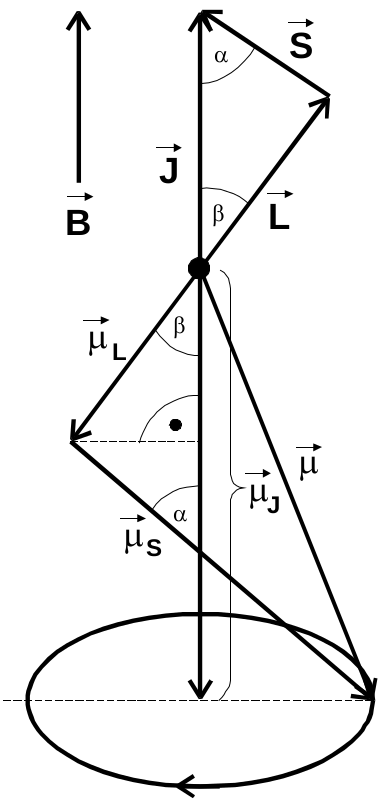
\includegraphics[height=5.5cm]{content/pictures/MagnMoment.png}
  \caption{Skizze zur Veranschaulichung der Zusammenhänge für die Bestimmung des magnetischen Moments der Elektronenhülle \cite{anleitung}.}
  \label{fig:magnmoment}
\end{figure}

\subsection{Magnetisches Moment des Atoms}
\label{sec:atom}
Neben den Hüllenelektronen trägt auch der Kern mit seinem Kernspin $I$ zum Gesamtdrehimpuls des Atoms $F$ bei.
Dabei verläuft dies analog zu Abschnitt \ref{sec:atomhülle}, genauer
\begin{equation*}
  \vec{F} = \vec{J} + \vec{I}.
\end{equation*}
Auf Grund der Kopplung vom Kernspin mit dem Gesmatdrehimpuls der Atomhülle ergibt sich die Aufspaltung der 
Hyperfeinstruktur, dabei darf das äußere Magnetfeld allerdings nicht zu stark sein.
Es ergeben sich $2J+1 (J<I)$ beziehungsweise $2I+1 (I<J)$  Unterniveaus. Dies Unterniveaus werden mit Hilfe
der Quantenzahl $F = |I-J|, \ldots,I+J-1, I+J$ unterschieden. Es spalten sich also zunächst die Feinstrukturniveaus
in die Hyperfeinstrukturniveaus auf, welche unter dem Einfluss eines äußeren Magnetfelds weiter in die 
Zeeman-Niveaus aufspalten. Die Energiedifferenz der Zeeman-Niveaus ergibt sich zu
\begin{equation}
  \label{eqn:zeeman}
  U_\text{Z} = g_\text{F} \mu_\text{B} |\vec{B}|.
\end{equation}
Mit Hilfe des magnetischen Moments des Atoms
\begin{equation*}
  \vec{\mu_text{F}} = -g_\text{F} \mu_\text{B} \vec{F}
\end{equation*}
und der richtungsorientierten Addition der Beträge der magnetischen Momente von Atomkern und Atomhülle
ergibt sich der Landé-Faktor
\begin{equation}
  \label{eqn:lande}
  g_\text{F} = g_\text{J} \frac{F(F+1)+J(J+1)-I(I+1)}{2F(F+1)}.
\end{equation}

\subsection{Optisches Pumpen}
\label{sec:pumpen}
Als optisches Pumpen wird eine Umbesetzung der thermischen Besetzung der Energieniveaus bezeichnet.
Um dieses Pumpen zu ermöglichen wird die in Abschnitt \ref{sec:atomhülle} beschriebene Zeeman-Aufspaltung benötigt.
Für ein Alkaliatome ergibt sich im Grundzustand ein $\ce{^{2}S\sfrac{1}{2}}$ Niveau, sowie die Niveaus
${}^2\text{P}_\sfrac{1}{2}$ und ${}^2\text{P}_\sfrac{3}{2}$ für den ersten angeregten Zustand, wenn der
Kerndrehimpuls vernachlässigt wird. Abbildung \ref{fig:aufspaltung} zeigt die Zeeman-Aufspaltung in die Zeeman-Niveaus für
die beiden Zustände mit $J=\sfrac{1}{2}$, also den optischen $\text{D}_1$-Übergang. Unter zu Hilfe nahme der Auswahlregeln für erlaubte Übergänge
\begin{align*}
  \Delta L & = \pm 1 \\
  \Delta M_\text{J} & = 0, \pm 1
\end{align*}
\begin{figure}
  \centering
  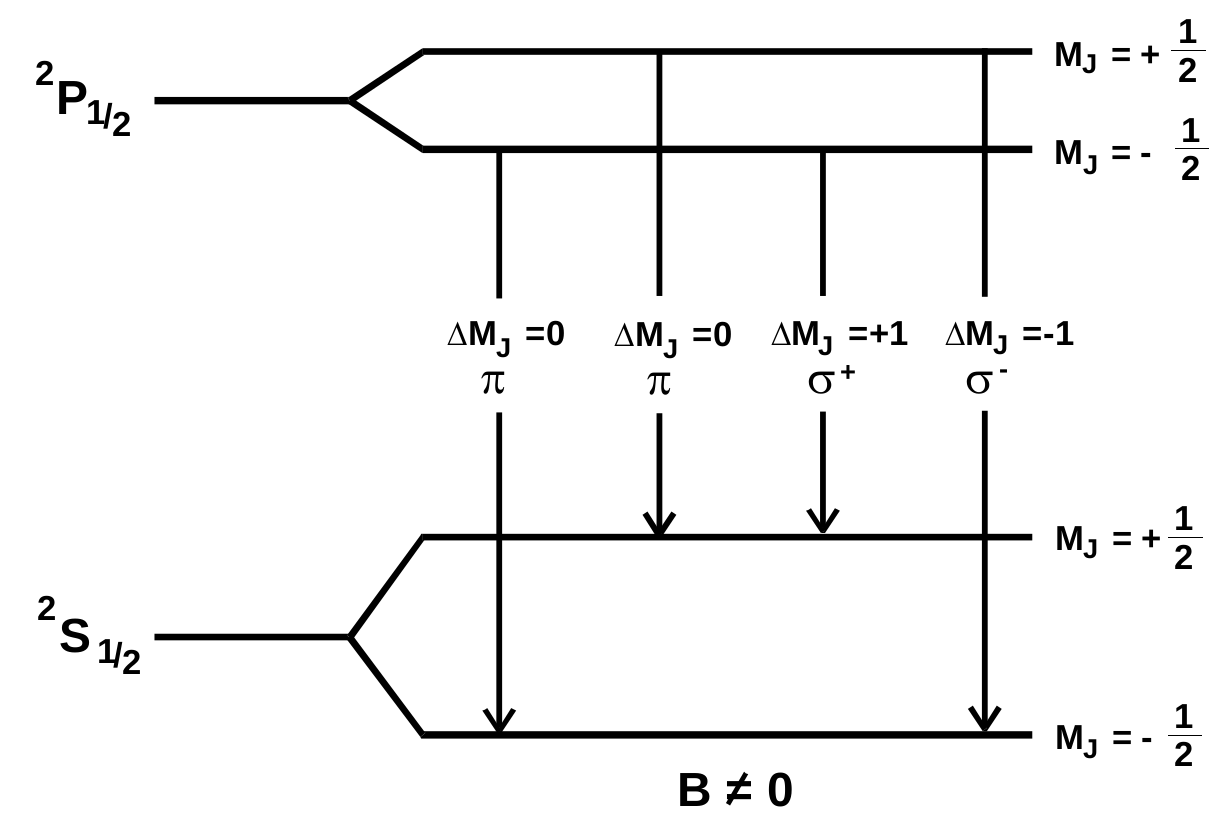
\includegraphics[height=5.5cm]{content/pictures/Energieniveaus.png}
  \caption{Die Energieniveau-Aufspaltung unter Einfluss eines $\vec{B}$-Feldes \cite{anleitung}.}
  \label{fig:aufspaltung}
\end{figure}
ergeben sich die in Abbildung \ref{fig:aufspaltung} als Pfeile eingezeichneten Übergänge.
Diese unterscheiden sich in Polarisation und Energie der ausgesendeten Quanten. So entspricht 
rechtszirkular-polarisiertes Licht, in Richtung von $\vec{B}$ ausgesendet dem $\sigma^+$-Übergang und 
linkszirkular-polarisiertes Licht dem $\sigma^-$-Übergang. Bei den $\pi$-Übergängen 
handelt es sich um emittiertes beziehungsweise absorbiertes Licht, welches linear-polarisiert
(parallel zu $\vec{B}$) ist und senkrecht zu $\vec{B}$ abgestrahlt wird.
Wird eine Dampfzelle bei der Temperatur $T$ mit einem Dampf aus Alkaliatomen befüllt und durchsetzt
dieses mit einem Magnetfeld so befinden sich die Atome zunächst im Grundzustand. Nun wird rechtszirkular-polarisiertes
$\text{D}_1$-Licht eingestrahlt und damit der Übergang mit $\Delta M_\text{J} = +1$ ermöglicht. 
Dadurch werden die Elektronen aus dem ${}^2\text{S}_\sfrac{1}{2}$-Niveau mit $M_\text{J}=\sfrac{-1}{2}$ in das 
${}^2\text{P}_\sfrac{1}{2}$-Niveau mit $M_\text{J}=\sfrac{1}{2}$ angehoben. Da es für die Emission
keine weiteren Einschränkungen gibt, finden beide Übergänge ins Grundniveau statt. Da aber immer nur
Elektronen aus dem Niveau mit $M_\text{J}=\sfrac{-1}{2}$ angeregt werden und kein Übergang inerhalb des
${}^2\text{S}_\sfrac{1}{2}$-Niveaus erlaubt ist, reichern sich die Elektronen im Niveau mit 
$M_\text{J}=\sfrac{1}{2}$ an und das mit $M_\text{J}=\sfrac{-1}{2}$ wird entleert. Somit ergibt sich eine 
nicht nach \eqref{eqn:boltz} gegebene thermische Besetzung. 
Mit Hilfe einer Photozelle auf der anderen Seite der Zelle wir die Transparenz des Gases beobachtet.
Wird das ${}^2\text{S}_\sfrac{1}{2}$-Niveau ($M_\text{J}=\sfrac{1}{2}$) entleert, so wird kein $\text{D}_1$-Licht
mehr absorbiert und die Intensität steigt an. Dieser Verlauf ist exemplarisch in Abbildung \ref{fig:intensität}
dargestellt.
\begin{figure}
  \centering
  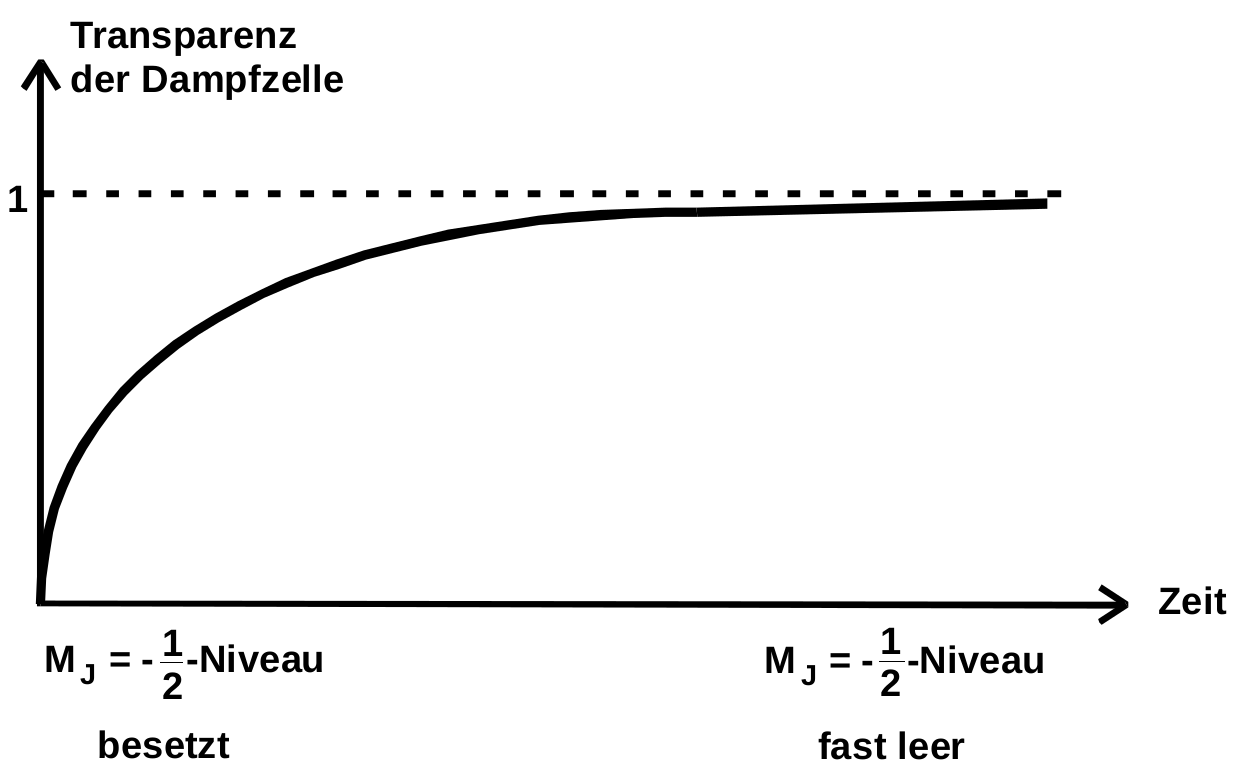
\includegraphics[height=5.5cm]{content/pictures/Transparenz.png}
  \caption{Exemplarischer Verlauf für die Transparenz der Dampfzelle in Abhängigkeit der Zeit \cite{anleitung}.}
  \label{fig:intensität}
\end{figure}

\FloatBarrier
% \begin{figure}
%   \centering
%   \includegraphics[height=5.5cm]{content/pictures/Bild.png}
%   \caption{Bilduterschrift}
%   \label{fig:Bild}
% \end{figure}

% \subsection{Unterkapitel}
% \label{sec:UnterKapitel}

% \begin{equation}
% Für Formeln
%   \label{eqn:Formel}
% \end{equation}
